%%=============================================================================
%% Stage-logboek
%%=============================================================================

\section{Stagedagboek}
\label{sec:stagedagboek}

\subsection{Week 1}

\subsubsection{Maandag 21/02/2022}

\emph{Eerste stagedag}. Kennismaking met \textbf{Tom De Leeuw}, Tom
staat in voor het linuxgedeelte. Laptop ontvangen, vooral gepraat over mogelijkheden van de stage.

Werkwijze voor telewerken:

\begin{enumerate}
    \item Surf naar \url{https://portal.connect.mil.be} en meld aan met \textbf{itsme}
    \item Kies voor vpn. Eens de verbinding opstaat kan je beginnen met skype.
\end{enumerate}

\subsubsection{Dinsdag 22/02/2022}

werkuren: \emph{8:00 - 16:00}

Zelfstandig research gedaan naar \gls{lvm}. \url{https://access.redhat.com/documentation/en-us/red_hat_enterprise_linux/8/html/configuring_and_managing_logical_volumes/index}

Na de research enkele kleine opdrachtjes uitgevoerd op mijn eigen devserver binnen Defensie:

\begin{enumerate}
    \item aanmaken logical volume
    \begin{itemize}
        \item maak logical volume aan van 300mb
        \item mount logical volume op \texttt{/var/data01}
        \item herstart server en kijk of het nog bestaat.
    \end{itemize}
    \item aanpassen logical volume
    \begin{itemize}
        \item vergroot logical volume
        \item verklein logical volume
    \end{itemize}
    \item volume groups
    \begin{itemize}
        \item maak 2 volume groups van 100-200mb
    \end{itemize}
\end{enumerate}

Achteraf als afsluiter van de dag moest ik een grafische omgeving installeren op mijn devserver en proberen om via windows \gls{rdp} de server te kunnen overnemen.

\subsubsection{Woensdag 23/02/2022}

werkuren: \emph{8:00 - 16:00}

Zelfstandig research gedaan naar
\href{https://www.redhat.com/en/technologies/management/satellite}{Redhat
    Satellite}, \href{https://theforeman.org}{Foreman} en
\href{https://www.theforeman.org/plugins/katello/}{Katello}. Ook naar
filesecurity: \glspl{acl}, \gls{selinux}.

Verworven kennis toegepast in demo-omgeving. Samen met Tom de Satellite
omgeving ontdekt. Uitleg gekregen hoe alles werkt.

\subsubsection{Donderdag 24/02/2022}

werkuren: \emph{8:00 - 16:00}

Kennis opgefrist ivm Mariadb, mysql en appstreams in RHEL. Manueel
mariadb geïnstalleerd op devmachine, \gls{db} en users aangemaakt. Research
over puppet en aan de hand van puppet mariadb proberen installeren en
users en \glspl{db} aan te maken. Meeting bijgewoond met externe mensen.

\subsection{Week 2}

\subsubsection{Maandag 28/02/2022}

werkuren: \emph{08:00-16:00}

Afgewerkt waar ik vorige donderdag mee bezig was. Bezig aan het
moderniseren van het script \texttt{bu\_script.sh}.

\subsubsection{Dinsdag 01/03/2022}

werkuren: \emph{8:00 - 16:00}

\texttt{bu\_script.sh} afgewerkt. Eenvoudige zelfgeschreven versie.\\
Begin aan voorbereiding theorie voor donderdag.

\subsubsection{Woensdag 02/03/2022}

werkuren: \emph{8:00 - 16:00}

Voorbereiding voor Donderdag

\begin{itemize}
    \item research gedaan in verband met \href{https://www.zabbix.com/documentation/5.0/en/manual/introduction/about}{Zabbix} (monitoring tool)
    \item git kennis opgefrist
    \item toegang gekregen tot de gitlab servers van Defensie.
    \item hello world project geschreven in Puppet op mijn dev machine
\end{itemize}

\subsubsection{Donderdag 03/03/2022}

werkuren: \emph{8:00 - 16:00}

Introductie tot Zabbix en puppet door Donovan. Daarna zelf via puppet
zabbix proberen installeren op devmachine.

\subsection{Week 3}

\subsubsection{Maandag 07/03/2022}

werkuren: \emph{08:00-16:00}

\begin{itemize}
    \item denk oefening:    
    \begin{itemize}
        \item hoe kan je het \texttt{bu\_script.sh} uitbreiden zodat er een melding komt in Zabbix wanneer een backup faalt?
        \item zoek uit wat er misgegaan is met de devmachine (te weinig geheugen).
    \end{itemize}
\end{itemize}

\subsubsection{Dinsdag 08/03/2022}

werkuren: \emph{8:00 - 16:00}

Introductie in Jboss applicatie servers door Christophe. Christophe
heeft me alles goed uitgelegd en we hebben een testapplicatie gedeployed
op mijn devmachine. Ik heb (onder begeleiding van Christophe) een
applicatie mogen vernieuwen in de acceptatieomgeving. (netmanto)

\subsubsection{Woensdag 09/03/2022}

werkuren: \emph{8:00 - 16:00}

De introductie in Jboss Applicatie servers verder gezet en afgewerkt. We
hebben nu niet alles maar redelijk veel overlopen van jboss servers. Ook
is het nu duidelijk hoe deze gemonitord worden (Jboss Operations
Networks).

Een eerste stagegesprek.

\subsubsection{Donderdag 10/03/2022}

Werkuren: \emph{08:30 - 16:30}

Werkdag in Peutie.

De opdracht gekregen om een oplossing te zoeken voor volgende problemen:

\begin{itemize}
    \item hoe high availability implementeren voor een db die aan een applicatie hangt?
    \item maak een procedure om Mariadb 5.5 op RHEL 7.x to upgraden naar Mariadb 10.6 op RHEL 8 zonder verlies van gegevens.
\end{itemize}

Ook de toegangsbadge in orde gemaakt samen met Donovan.

\subsection{Week 4}

\subsubsection{Maandag 14/03/2022}

werkuren: \emph{08:00-16:00}

Verder gewerkt aan de denkoefeningen op een iteratieve manier. Alles
mooi in een word-documentje gegoten.

\subsubsection{Dinsdag 15/03/2022}

werkuren: \emph{8:00 - 16:00}

Verder gewerkt aan de denkoefeningen op een iteratieve manier. Er is
nood aan validatie van gebruikers en databanken. Hiervoor een concept
bedacht.

\subsubsection{Woensdag 16/03/2022}

werkuren: \emph{8:00 - 16:00}

Verder gewerkt aan de denkoefeningen.

Upgrade mariadb:

\begin{itemize}
    \item validatie voor users bedacht. gestart aan een script om dit uit te
    voeren maar ik zat vast gaandeweg dus nu ga ik eens kijken dat er geen
    andere manier is om dit te doen.
\end{itemize}

db high availability:

\begin{itemize}
    \item iteratie afgewerkt. Nu wachten op feedback.
\end{itemize}

Stageverslag: structuur opgemaakt.

\subsubsection{Donderdag 17/03/2022}

Werkuren: \emph{08:15 - 16:15}

Fysiek in Peutie.

Normaal was er een introductie van \gls{mssql} gepland vandaag maar deze is
verzet naar een later moment. Ter vervanging heb ik verschillende
praktische oefeningen gedaan ivm \gls{lvm} op mijn devmachine. Ook dit
allemaal besproken met Tom.

\subsection{Week 5}

\subsubsection{Maandag 21/03/2022}

werkuren: \emph{08:00-16:00}

Verder gewerkt aan de denkoefening om high availability te implementeren
bij databanken. Tom heeft voor mij een aantal virtuele machines laten
maken zodat ik hierop kan testen.

Stageverslag verder aangevuld.

\subsubsection{Dinsdag 22/03/2022}

Geen stage.\\
Jobevent van HoGent


\subsubsection{Woensdag 23/03/2022}

werkuren: \emph{8:00 - 16:00}

Verder gewerkt aan de denkoefening om high availability te implementeren
bij databanken: Testopstelling gemaakt.

\begin{itemize}
    \item
    databank master
    \item
    databank slave
    \item
    reverse proxy
\end{itemize}

Zie Figuur \ref{fig:netwerkdiagram-db-replicatie}, Dit is het netwerkdiagram van de opstelling.

\begin{figure}
    \centering
    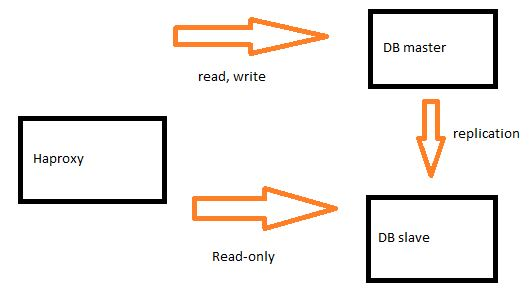
\includegraphics{img/networkdiagram_db_replication.JPG}
    \caption{\label{fig:netwerkdiagram-db-replicatie}netwerk diagram}
\end{figure}

Er is nog uitbreiding mogelijk: Hoe van replica een master maken?

\subsubsection{Donderdag 24/03/2022}

Fysiek in Peutie

werkuren: \emph{8:00 - 16:00}

Introductie van \emph{\gls{mssql}}\\
Onderzoeksopdracht besproken. ik zal hierover nog een document
ontvangen.\\
Tom heeft mij een rondleiding gegeven in de serverroom van in Peutie.

In de namiddag was er een drink binnen defensie waar de kolonel een
toespraak heeft gehouden. Het was tof om deze bij te wonen.

\subsection{Week 6}

\subsubsection{Maandag 28/03/2022}

werkuren: \emph{08:00-16:00}

Gewerkt aan de opdracht voor \gls{mssql}. Vooral research gedaan en mezelf
bekend gemaakt met het onderwerp. Ook een virtuele machine gevraagd om dingen te testen.


\subsubsection{Dinsdag 29/03/2022}

werkuren: \emph{08:00-16:00}

Bijlagen toegevoegd aan stageverslag. Verder onderzoek gedaan voor \gls{mssql}.
Gewacht op de virtuele machine.

Ad hoc een taak gekregen van Tom: schrijf een patch voor een databank. zie bijlage \ref{subsec:tables_patch}

\subsubsection{Woensdag 30/03/2022}

werkuren: \emph{08:00-16:00}

Blijkbaar is het niet simpel om voor mij een virtuele machine te voorzien dus we hebben het het opgelost door een named instance te maken op een bestaande server. Hierdoor heb ik enkele dingen kunnen testen in \gls{mssql}.

\subsubsection{Donderdag 31/03/2022}

werkuren: \emph{08:00-16:00}

Telewerken.

Verder gewerkt aan de opdracht van \gls{mssql}. Begonnen aan een script te schrijven voor de conversie van de logins/users te doen.  
Dit is moeilijker dan ik gedacht had.

\subsection{Week 7}

\subsubsection{Maandag 04/04/2022}

werkuren: \emph{08:00-16:00}

Verder gewerkt aan de opdracht van \gls{mssql}, niet gemakkelijk. Men kan zeggen dat ik vast zit.  
Johan was niet online dus ik kon hem niet bereiken om hulp te vragen.

\subsubsection{Dinsdag 05/04/2022}

werkuren: \emph{08:00-16:00}

Verder gewerkt aan de opdracht. Zit nog steeds vast, Johan niet online.

\subsubsection{Woensdag 06/04/2022}

werkuren: \emph{08:00-16:00}

Hulp gevraagd aan Johan maar nog geen antwoord gekregen. Voor de rest verder gewerkt aan de opdracht van \gls{mssql}.

\subsubsection{Donderdag 07/04/2022}

werkuren: \emph{08:00-16:00}

Telewerken.

Verder gewerkt aan \gls{mssql}.

\subsection{Week 8}

\subsubsection{Maandag 11/04/2022}

Afwezig

\subsubsection{Dinsdag 12/04/2022}

Afwezig

\subsubsection{Woensdag 13/04/2022}

Afwezig

\subsubsection{Donderdag 14/04/2022}

Afwezig

\subsection{Week 9}

\subsubsection{Maandag 19/04/2022}

geen stage. (paasmaandag)

\subsubsection{Dinsdag 20/04/2022}

werkuren: \emph{08:00-16:00}

Verder gewerkt aan de opdracht van \gls{mssql}. Ik zit hierin vast en ik heb nog geen contact kunnen maken met Johan. Tom had vandaag geen tijd om mij te helpen maar zal morgen contact opnemen met mij.

\subsubsection{Woensdag 21/04/2022}

werkuren: \emph{10:00-17:00}

Stand van zaken voor de opdracht van \gls{mssql} besproken met Tom. Johan heeft deze week nog verlof en zal vanaf volgende week terug aanwezig zijn. Contact gehad met Steven om een moment in te plannen om de mogelijkheden na de stage te bespreken.

\subsubsection{Donderdag 22/04/2022}

werkuren: \emph{08:00-16:00}

Begonnen aan het script om de users te checken voor de opdracht mysql migratie.

\subsection{Week 10}

\subsubsection{Maandag 25/04/2022}

werkuren: \emph{08:15-16:15}

Contact gehad met Johan en Donovan over de opdracht van \gls{mssql}. Meer info gezocht over de jtds driver. ook naar de jdbc driver gekeken.

\subsubsection{Dinsdag 26/04/2022}

werkuren: \emph{08:15-16:15}

Verder gewerkt aan de oefening van \gls{mssql}: meer info gezocht over de jtds en jdbc drivers. niet gevonden wat ik wou vinden.

Om mijn gedachten eens te verzetten heb ik nog eens gekeken naar het script `check\_users.py` en heb ik de output een aangepast zodat er nu een waarschuwing staat en verder gescrheven aan het stageverslag.

Voor de opdracht High availability voor mariadb: Research gedaan over hoe we in plaats van master-slave naar master-master kunnen gaan.


\subsubsection{Woensdag 27/04/2022}

werkuren: \emph{10:00-17:30}

Verder gezocht naar een oplossing voor de jtds driver. Steeds niet gevonden, morgen ga ik hierover met Donovan proberen praten om samen een oplossing te zoeken.
Nagedacht over hoe ik een testopstelling ga opzetten voor een master-master opstelling bij de opdracht High availability voor mariadb.
Stageverslag verder aangevuld.

\subsubsection{Donderdag 28/04/2022}

werkuren: \emph{8:15-16:15}

\subsection{Week 11}

\subsubsection{Maandag 02/05/2022}

\subsubsection{Dinsdag 03/05/2022}

\subsubsection{Woensdag 04/05/2022}

\subsubsection{Donderdag 05/05/2022}

\subsection{Week 12}

\subsubsection{Maandag 09/05/2022}

\subsubsection{Dinsdag 10/05/2022}

\subsubsection{Woensdag 11/05/2022}

\subsubsection{Donderdag 12/05/2022}

\subsection{Week 13}

\subsubsection{Maandag 16/05/2022}

\subsubsection{Dinsdag 17/05/2022}

\subsubsection{Woensdag 18/05/2022}

\subsubsection{Donderdag 19/05/2022}

\subsection{Week 14}

\subsubsection{Maandag 23/05/2022}

\subsubsection{Dinsdag 24/05/2022}

\subsubsection{Woensdag 25/05/2022}

\subsubsection{Donderdag 26/05/2022}